\chapter{Implementacja obiektu}

Pierwszym zadaniem do wykonania podczas tej części projektu była implementacja zadanego obiektu w środowisku OVATION. Zanim jednak przystąpiliśmy do implementacji należało przekształcić model z równań ciągłych na dyskretne. Zgodnie z instrukcją podaną przez prowadzącego zostało to wykonane poprzez proste podstawienie, w którym k to numer kroku modelu, a $T_S$ oznacza czas próbkowania:

\begin{equation}
\left\{
\begin{tabular}{l}
$\frac{dC_A}{dt} = \frac{C_{A_{k+1}}-C_{A_k}}{T_s}$\\
$\frac{dT}{dt} = \frac{T_{k+1}-T_k}{T_s}$
\end{tabular}
\right.
\end{equation}

Jako czas próbkowania przyjęliśmy 1 sekundę. Ponieważ jednak nasz obiekt posługuje się nominalnie minutami wartość $T_s$ wyniosła 1/60. Ostatecznie więc do implementacji otrzymaliśmy następujące równania:

\begin{equation}
\left\{
\begin{tabular}{l}
$C_{A_{k+1}} = (C_{Ain_k} - C_{A_k} - 10^{10}\cdot e^{-\frac{8330,1}{T_k}}\cdot C_{A_k})/60+C_{A_k}$\\
$T_{k+1} =( T_{in_k} - T_k + 130\cdot 10^{10}\cdot e^{-\frac{8330,1}{T_k}}\cdot C_{A_k}-\frac{1,678\cdot (F_{C_k})^{1,5}}{F_{C_k}+0,839\cdot (F_{C_k})^{0,5}}(T_k-T_{Cin_k}))/60+T_k$
\end{tabular}
\right.
\end{equation}

Mając tak przygotowane wzory przystąpiliśmy do implementacji, którą zaczęliśmy od utworzenia odpowiednich punktów wejściowych (4 punkty: 2 dla sterowania i 2 dla zakłóceń) i wyjściowych (2 punkty). Utworzone zostały punkty o następujących nazwach:
\begin{itemize}
	\item 3\_CAIN\_IN
	\item 3\_FC\_IN
	\item 3\_TIN\_IN
	\item 3\_TCIN\_IN
	\item 3\_CA\_OUT
	\item 3\_T\_OUT
\end{itemize}
Punkty odpowiadające sterowaniom oraz wyjściom obiektu zostały następnie przypisane odpowiednio do bloków wejść i wyjść wewnątrz arkusza projektowego. Punkty zakłóceń zadane zostały poprzez użycie bloków AVALGEN. Dodatkowo sterowania podłączone zostały poprzez blok TRANSFER sterowany sygnałem binarnym. Blok ten określa czy w danej chwili regulator pracuje w trybie ręcznym czy też automatycznym.

Po umieszczeniu wejść oraz wyjść modelu na arkuszu nadeszła pora na implementację samego obiektu. W tym celu wykorzystaliśmy bloki CALCBLOCK umożliwiające dokonywanie obliczeń z wykorzystaniem do 18 zmiennych wejściowych, z których to wejść nasz model wykorzystywał jedynie 6. Dla każdego użytego bloku, jako wejścia od IN1 do IN6 posłużyły nam kolejno: $C_{Ain}, F_C, T_{in}, T_{Cin}, C_A$ oraz $T$. Implementacja pierwszego równania obyła się bez przeszkód. Jest ona przedstawiona na poniższym rysunku.

\begin{figure}[h!]
	\centering
	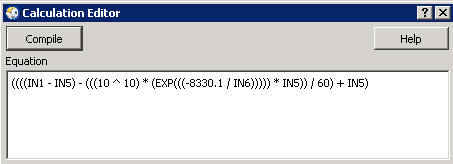
\includegraphics[width=.5\linewidth]{img/CALCBLOCK1.png}
	\label{ch1:calc1}
	\caption{Formuła pierwszego równania modelu wewnątrz CALCBLOCK}
\end{figure}

Niewielki problem wystąpił podczas implementacji równania drugiego wyjścia modelu. Ze względu na ograniczenie nałożone na ilość znaków mogących się znaleźć wewnątrz formuły bloku CALCBLOK, działanie to musiało być przez nas podzielone na dwa bloki. W pierwszym z nich umieszczony został fragment: $T_{in_k} - T_k + 130\cdot 10^{10}\cdot e^{-\frac{8330,1}{T_k}}\cdot C_{A_k}$. Pozostała część zmieściła się w drugim. W celu wyraźnego odgraniczenia wyjścia pierwszego bloku od zmiennych procesu, zostało one wprowadzone do drugiego bloku jako IN18. Obydwa bloki zostały także odpowiednio połączone, tak aby kalkulacje w bloku drugim zachodziły zawsze po kalkulacjach bloku pierwszego. Zawartość obydwu bloków przedstawiona została na rysunkach poniżej.

\begin{figure}[h!]
	\centering
	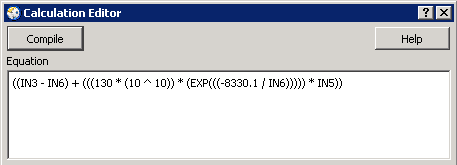
\includegraphics[width=.5\linewidth]{img/CALCBLOCK2.png}
	\label{ch1:calc2}
	\caption{Formuła wewnątrz pierwszego bloku CALCBLOCK dla drugiego równania modelu}
\end{figure}

\begin{figure}[h!]
	\centering
	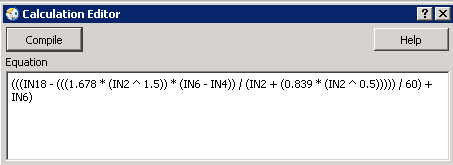
\includegraphics[width=.5\linewidth]{img/CALCBLOCK3.png}
	\label{ch1:calc3}
	\caption{Formuła wewnątrz drugiego bloku CALCBLOCK dla drugiego równania modelu}
\end{figure}

Po odpowiednim połączeniu wszystkich elementów otrzymaliśmy działający model zadanego dla nas obiektu. W celu jego przetestowania wykonaliśmy skok sterowania $C_{Ain}$ do wartości 1,6. Obiekt zachował się zgodnie z oczekiwaniami, a wartości wyjścia zbiegły do oczekiwanych. Poniżej zamieszczamy wykresy otrzymane w wyniku tego testu.

\begin{figure}[h!]
	\centering
	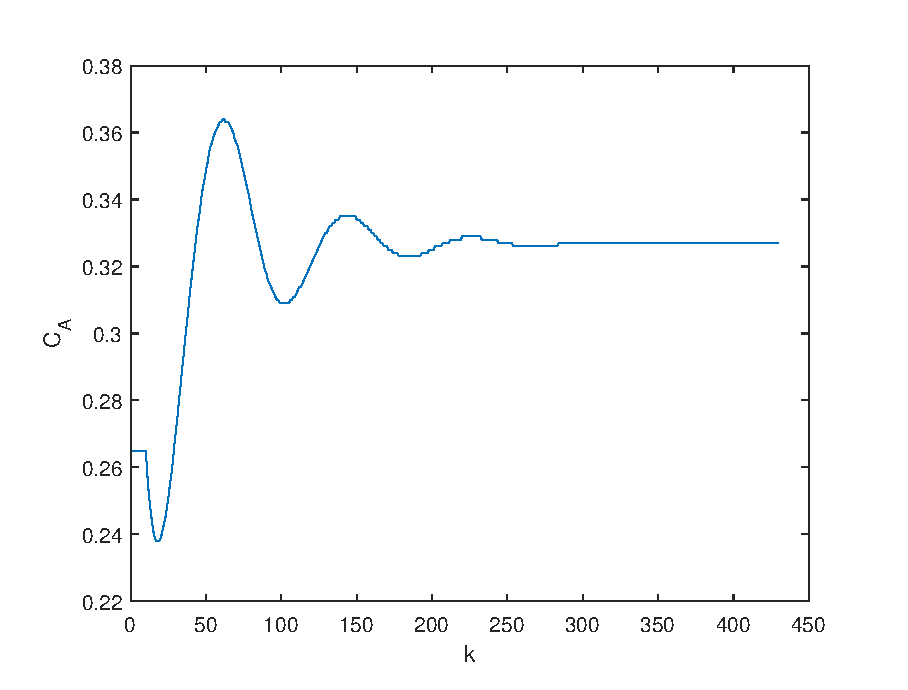
\includegraphics[width=.8\linewidth]{img/model1.eps}
	\label{ch1:model1}
	\caption{Wyjście $C_A$ modelu po skoku sterowania $C_{Ain}$ do 1,6}
\end{figure}

\begin{figure}[h!]
\centering
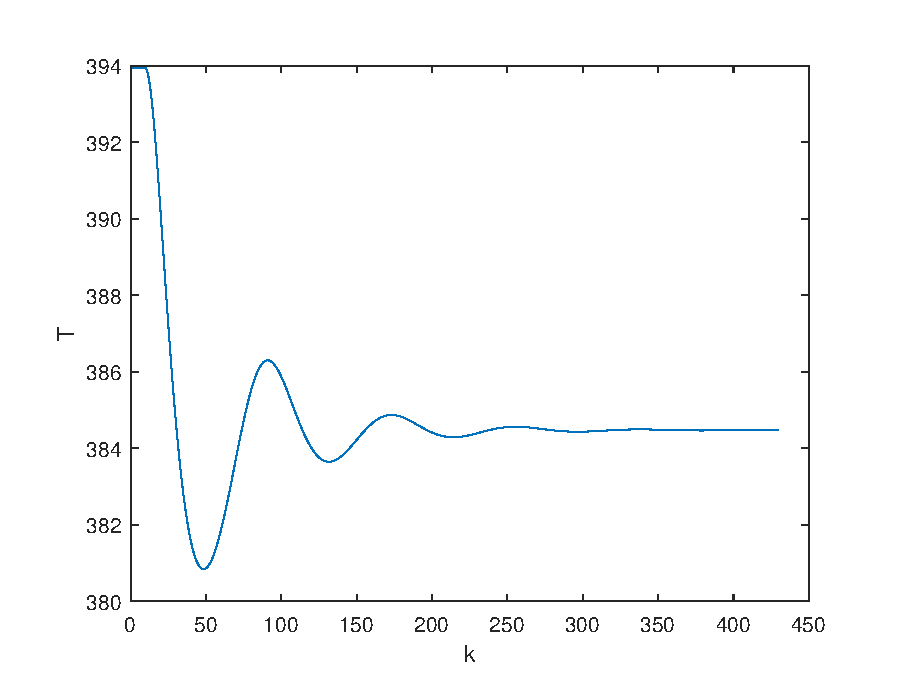
\includegraphics[width=.8\linewidth]{img/model2.eps}
\label{ch1:model2}
\caption{Wyjście $T$ modelu po skoku sterowania $C_{Ain}$ do 1,6}
\end{figure}

\begin{figure}[h!]
	\centering
	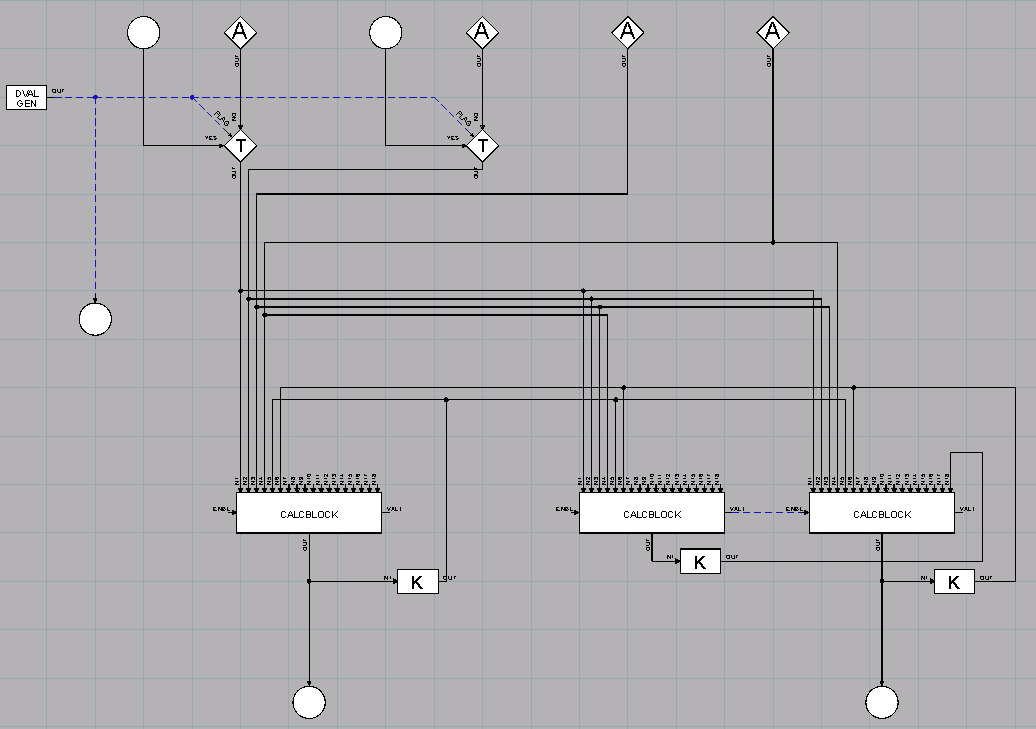
\includegraphics[width=\linewidth]{img/MODEL.png}
	\label{ch1:model}
	\caption{Model obiektu wykonany w programie OVATION}
\end{figure}